\providecommand{\main}{..}
\documentclass[../cmpe-251-project-report.tex]{subfiles}
\externaldocument{1-introduction}
\externaldocument{2-dataset-properties}
\externaldocument{3-attribute-selection-ranking}
\externaldocument{5-predictors}
\externaldocument{6-actionable-conclusions}

\begin{document}
  \chapter{Clustering}
  \label{ch:clustering}
  Both \(k\)-means and Singular Value Decomposition (SVD) methods of clustering were used to determine more properties from the data, using only the important attributes discussed in \cref{ch:selection-ranking}.

  \section{Singular Value Decomposition}
  SVD clustering was attempted first to help visualize potential clusters and to further analyze the correlation between different attributes. From \cref{subfig:svd-revenue-clustering}, there is an evident separation between data points in either of the Revenue's classes. So clustering using \(k\)-means should be feasible given the observed clumpiness, but may require multiple clusters due to how close the groups are. The Figure also shows promise for an accurate prediction model given the grouping of the two classes.
  \begin{figure}
    \begin{subfigure}[t]{0.49\textwidth}
      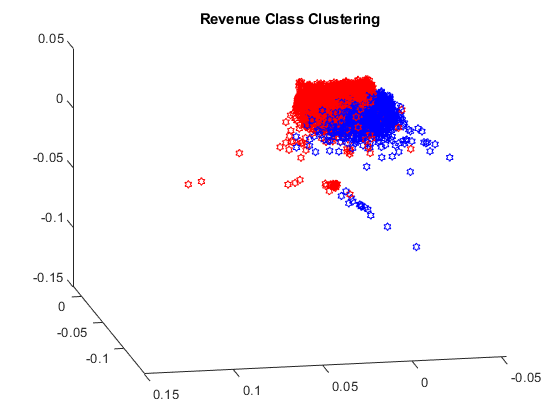
\includegraphics[width=\textwidth]{svd-revenue-clustering.png}
      \subcaption{SVD clustering of data points coloured based on Revenue class.\\Blue = TRUE, Red = FALSE.}
      \label{subfig:svd-revenue-clustering}
    \end{subfigure}
    \begin{subfigure}[t]{0.49\textwidth}
      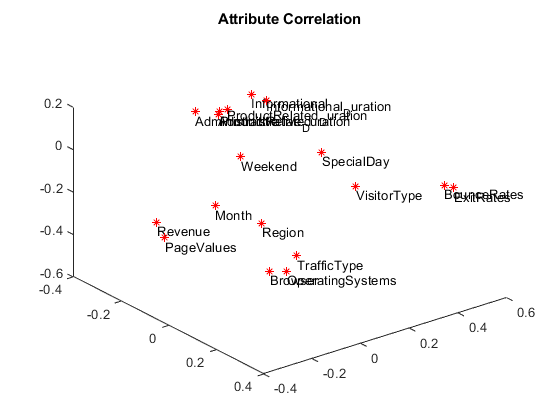
\includegraphics[width=\textwidth]{svd-attribute-correlation.png}
      \subcaption{SVD of the attributes.}
      \label{subfig:svd-attribute-correlation}
    \end{subfigure}
    \caption{SVD figures generated from a modified version of the \texttt{showsvd.m} MATLAB script.}
  \end{figure}
  In addition, \cref{subfig:svd-attribute-correlation} shows that the Revenue and Page Values attributes are highly correlated, which reinforces the correlation analysis conducted in \cref{ch:dataset-properties} and the attribute ranking done in \cref{ch:selection-ranking}. There is also some strong correlation between the important attributes located in different ``correlation'' clusters. The more notable of those clusters is the Bounce Rate and Exit Rate attributes being isolated and correlated similarly to the Revenue and Page Values attributes. This has some implications for the website's page structure, which will be further discussed in \cref{ch:actionable-conclusions}.

  \section{\(k\)-Means}
  After trying various values of \(k\) in the range of \([2,7]\), the number of clusters that provided the most useful insight was 4. From \cref{fig:scatter-plot-k-means}, we can see that the clusters 0 and 3 reveal that revenue generating visitors do tend to have high Page values and low Exit Rates associated. The reverse trend can be observed in clusters 1 and 2, which reinforces the correlation analysis conducted in \cref{ch:dataset-properties}.
  \begin{figure}
    \begin{subfigure}{0.49\textwidth}
      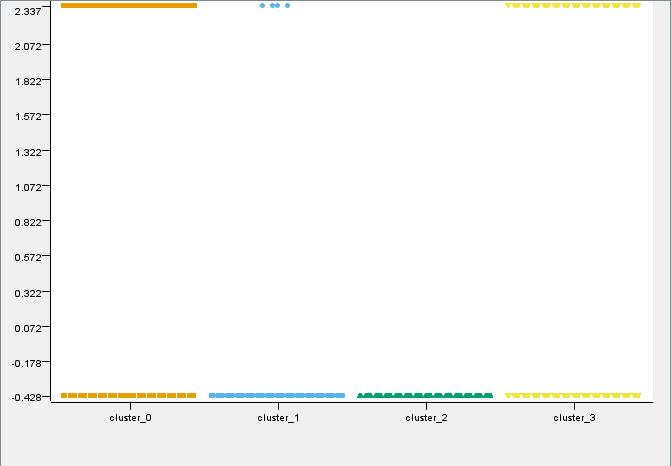
\includegraphics[width=\textwidth]{scatter-plot-clusters-revenue.png}
      \caption{Clusters vs. Revenue}
    \end{subfigure}
    \begin{subfigure}{0.49\textwidth}
      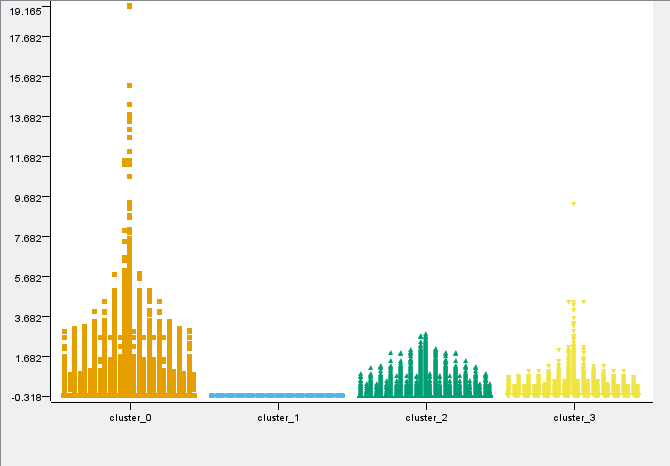
\includegraphics[width=\textwidth]{scatter-plot-clusters-page-values.png}
      \caption{Clusters vs. Page Values}
    \end{subfigure}
    \par\bigskip
    \begin{subfigure}{0.49\textwidth}
      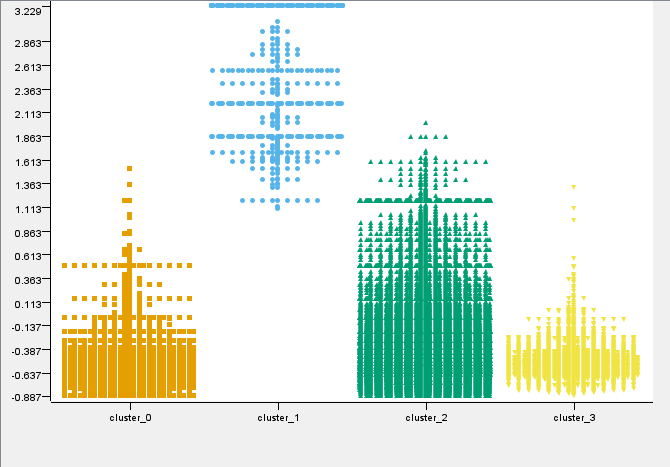
\includegraphics[width=\textwidth]{scatter-plot-clusters-exit-rates.png}
      \caption{Clusters vs. Exit Rates}
    \end{subfigure}
    \caption{Scatter plots of the \(k\)-means clusters against significant attributes.}
    \label{fig:scatter-plot-k-means}
  \end{figure}
  One may want to target clusters 1 and 2 to determine what would make them purchase something from Nozama's website, which will be expanded on in \cref{ch:actionable-conclusions}.
\end{document}
